\documentclass[a4paper,12pt]{article}

\usepackage[T2A]{fontenc}
\usepackage[utf8]{inputenc}
\usepackage[russian,english]{babel}

\usepackage{cmap}
\usepackage{minted}
\usepackage{subfigure}
\usepackage{wrapfig}
\usepackage{indentfirst}
\usepackage{autonum}
\usepackage{amsfonts}
\usepackage{amsmath}
\usepackage{amssymb}
\usepackage{amsthm}
\usepackage{upgreek}
\usepackage{graphicx}
\usepackage{listings}
\usepackage{multirow}
\usepackage{multicol}
\usepackage{dsfont}
\usepackage{graphicx}
\usepackage{caption}
\usepackage{stmaryrd}
\usepackage{setspace,amsmath}
\usepackage{lipsum}
\usepackage{mwe}
\usepackage[nottoc,notlot,notlof]{tocbibind}

\linespread{1.25}
% \setlength\parindent{1.25ex}

\usepackage[unicode, pdftex]{hyperref}
\usepackage[left=20mm, top=20mm, right=15mm, bottom=20mm, footskip=15mm]{geometry}

\usepackage{xcolor}

\definecolor{maroon}{cmyk}{0, 0.87, 0.68, 0.32}
\definecolor{halfgray}{gray}{0.55}
\definecolor{ipython_frame}{RGB}{207, 207, 207}
\definecolor{ipython_bg}{RGB}{247, 247, 247}
\definecolor{ipython_red}{RGB}{186, 33, 33}
\definecolor{ipython_green}{RGB}{0, 128, 0}
\definecolor{ipython_cyan}{RGB}{64, 128, 128}
\definecolor{ipython_purple}{RGB}{170, 34, 255}

\usepackage{listings}
\lstset{
    breaklines=true,
    texcl=true,
    %
    extendedchars=true,
    literate=
    {á}{{\'a}}1 {é}{{\'e}}1 {í}{{\'i}}1 {ó}{{\'o}}1 {ú}{{\'u}}1
    {Á}{{\'A}}1 {É}{{\'E}}1 {Í}{{\'I}}1 {Ó}{{\'O}}1 {Ú}{{\'U}}1
    {à}{{\`a}}1 {è}{{\`e}}1 {ì}{{\`i}}1 {ò}{{\`o}}1 {ù}{{\`u}}1
    {À}{{\`A}}1 {È}{{\'E}}1 {Ì}{{\`I}}1 {Ò}{{\`O}}1 {Ù}{{\`U}}1
    {ä}{{\"a}}1 {ë}{{\"e}}1 {ï}{{\"i}}1 {ö}{{\"o}}1 {ü}{{\"u}}1
    {Ä}{{\"A}}1 {Ë}{{\"E}}1 {Ï}{{\"I}}1 {Ö}{{\"O}}1 {Ü}{{\"U}}1
    {â}{{\^a}}1 {ê}{{\^e}}1 {î}{{\^i}}1 {ô}{{\^o}}1 {û}{{\^u}}1
    {Â}{{\^A}}1 {Ê}{{\^E}}1 {Î}{{\^I}}1 {Ô}{{\^O}}1 {Û}{{\^U}}1
    {œ}{{\oe}}1 {Œ}{{\OE}}1 {æ}{{\ae}}1 {Æ}{{\AE}}1 {ß}{{\ss}}1
    {ç}{{\c c}}1 {Ç}{{\c C}}1 {ø}{{\o}}1 {å}{{\r a}}1 {Å}{{\r A}}1
    {€}{{\EUR}}1 {£}{{\pounds}}1
}

%%
%% Python definition (c) 1998 Michael Weber
%% Additional definitions (2013) Alexis Dimitriadis
%% modified by me (should not have empty lines)
%%
\lstdefinelanguage{iPython}{
    morekeywords={access,and,break,class,continue,def,del,elif,else,except,exec,finally,for,from,global,if,import,in,is,lambda,not,or,pass,print,raise,return,try,while},%
    %
    % Built-ins
    morekeywords=[2]{abs,all,any,basestring,bin,bool,bytearray,callable,chr,classmethod,cmp,compile,complex,delattr,dict,dir,divmod,enumerate,eval,execfile,file,filter,float,format,frozenset,getattr,globals,hasattr,hash,help,hex,id,input,int,isinstance,issubclass,iter,len,list,locals,long,map,max,memoryview,min,next,object,oct,open,ord,pow,property,range,raw_input,reduce,reload,repr,reversed,round,set,setattr,slice,sorted,staticmethod,str,sum,super,tuple,type,unichr,unicode,vars,xrange,zip,apply,buffer,coerce,intern},%
    %
    sensitive=true,%
    morecomment=[l]\#,%
    morestring=[b]',%
    morestring=[b]",%
    %
    morestring=[s]{'''}{'''},% used for documentation text (mulitiline strings)
    morestring=[s]{"""}{"""},% added by Philipp Matthias Hahn
    %
    morestring=[s]{r'}{'},% `raw' strings
    morestring=[s]{r"}{"},%
    morestring=[s]{r'''}{'''},%
    morestring=[s]{r"""}{"""},%
    morestring=[s]{u'}{'},% unicode strings
    morestring=[s]{u"}{"},%
    morestring=[s]{u'''}{'''},%
    morestring=[s]{u"""}{"""},%
    %
    % {replace}{replacement}{lenght of replace}
    % *{-}{-}{1} will not replace in comments and so on
    literate=
    {á}{{\'a}}1 {é}{{\'e}}1 {í}{{\'i}}1 {ó}{{\'o}}1 {ú}{{\'u}}1
    {Á}{{\'A}}1 {É}{{\'E}}1 {Í}{{\'I}}1 {Ó}{{\'O}}1 {Ú}{{\'U}}1
    {à}{{\`a}}1 {è}{{\`e}}1 {ì}{{\`i}}1 {ò}{{\`o}}1 {ù}{{\`u}}1
    {À}{{\`A}}1 {È}{{\'E}}1 {Ì}{{\`I}}1 {Ò}{{\`O}}1 {Ù}{{\`U}}1
    {ä}{{\"a}}1 {ë}{{\"e}}1 {ï}{{\"i}}1 {ö}{{\"o}}1 {ü}{{\"u}}1
    {Ä}{{\"A}}1 {Ë}{{\"E}}1 {Ï}{{\"I}}1 {Ö}{{\"O}}1 {Ü}{{\"U}}1
    {â}{{\^a}}1 {ê}{{\^e}}1 {î}{{\^i}}1 {ô}{{\^o}}1 {û}{{\^u}}1
    {Â}{{\^A}}1 {Ê}{{\^E}}1 {Î}{{\^I}}1 {Ô}{{\^O}}1 {Û}{{\^U}}1
    {œ}{{\oe}}1 {Œ}{{\OE}}1 {æ}{{\ae}}1 {Æ}{{\AE}}1 {ß}{{\ss}}1
    {ç}{{\c c}}1 {Ç}{{\c C}}1 {ø}{{\o}}1 {å}{{\r a}}1 {Å}{{\r A}}1
    {€}{{\EUR}}1 {£}{{\pounds}}1,
    %
    literate=
    *{+}{{{\color{ipython_purple}+}}}1
    {-}{{{\color{ipython_purple}-}}}1
    {*}{{{\color{ipython_purple}$^\ast$}}}1
    {/}{{{\color{ipython_purple}/}}}1
    {^}{{{\color{ipython_purple}\^{}}}}1
    {?}{{{\color{ipython_purple}?}}}1
    {!}{{{\color{ipython_purple}!}}}1
    {\%}{{{\color{ipython_purple}\%}}}1
    {<}{{{\color{ipython_purple}<}}}1
    {>}{{{\color{ipython_purple}>}}}1
    {|}{{{\color{ipython_purple}|}}}1
    {\&}{{{\color{ipython_purple}\&}}}1
    {~}{{{\color{ipython_purple}~}}}1
    %
    {==}{{{\color{ipython_purple}==}}}2
    {<=}{{{\color{ipython_purple}<=}}}2
    {>=}{{{\color{ipython_purple}>=}}}2
    %
    {+=}{{{+=}}}2
    {-=}{{{-=}}}2
    {*=}{{{$^\ast$=}}}2
    {/=}{{{/=}}}2,
    %
    commentstyle=\color{ipython_cyan}\ttfamily,
    stringstyle=\color{ipython_red}\ttfamily,
    keepspaces=true,
    showspaces=false,
    showstringspaces=false,
    rulecolor=\color{ipython_frame},
    frame=single,
    frameround={t}{t}{t}{t},
    framexleftmargin=6mm,
    numbers=left,
    numberstyle=\tiny\color{halfgray},
    %
    backgroundcolor=\color{ipython_bg},
    % extendedchars=true,
    basicstyle=\scriptsize\ttfamily,
    keywordstyle=\color{ipython_green}\ttfamily,
    escapechar=\%,
    escapebegin=\color{ipython_green},
    texcl=true,
    inputencoding=utf8
}


\begin{document}
    \selectlanguage{russian}
    \pagestyle{empty}
    \vbox{%
        \hfill%
        \vbox{%
            \hbox{УДК XXX.XXX}%
            \hbox{\textbf{Гамосов C. C.}}%
            \hbox{Северо-Осетинский государственный университет}%
            \hbox{имени Коста Левановича Хетагурова,}%
            \hbox{362025, Россия, г. Владикавказ, ул. Церетели, 16,}%
            \hbox{gamosov.gs@yandex.ru}%
        }%
    }
    
    \begin{center}
        \Large{\textbf{Концепция Seq2Seq для нейронного перевода}}
    \end{center}
    
    \textbf{Ключевые слова:} Нейронный Машинный Перевод, Gated Recurrent Unit, Модель Seq2Seq, Attention, Осетинский язык.
    
    \section*{Введение}
    
	За последние годы качество моделей машинного перевода резко выросло, связано это с началом использования в них рекуррентных нейронных сетей (RNN). Они позволили снизить затраты на выявления лингвистических закономерностей языков и дорогостоящую разработку алгоритмов для их обработки, что использовалось в RBMT (Rule-Based Machine Translation). В свою очередь NMT (Neural Machine Translation) довольно хорошо справляется со своей задачей, но все таки ему до сих пор не удается полностью сместить SMT (Statistical Machine Translation). Хотя количество статистического перевода в современных переводчиках снизилось почти до минимума. Теперь уже при построении хорошей модели машинного перевода большую часть работы стоит сконцентрировать, на особенности языка, его структуре, связи между словами и их значениями. Решением данного перечня проблем и являются модели sequence-to-sequence (\cite{4}, \cite{5}, \cite{6}).
	
    Seq2Seq - это семейство подходов машинного обучения, используемых для обработки языка. Первоначальный подход Seq2Seq, который в процессе породил целое семейство методов, был разработан Google для использования в машинном переводе \cite{11}. Как уже можно заметить за последнюю пару лет коммерческие системы стали удивительно хороши в переводе - посмотрите, например, Google Translate, Яндекс-Переводчик, переводчик DeepL, переводчик Bing Microsoft. Данный подход хорош не только в нейронном переводе. Текстовое описание к изображению и обобщение (summarize) текста - вот не полный список задач, в которых используются данная модель.
	
	В статье рассматривается задача нейронного машинного перевода - NTM (Neural Machine Translation). Формальная цель поставленной проблемы - это перевод предложений c одного естественного языка на другой с помощью машины. Так же помимо теоретического описания, построения, были реализованы модели и проведен поверхностный анализ качества полученных результатов.
	
	\hfill
	
	{\footnotesize © Гамосов С.С., 2022}
	
	\clearpage
	
	\section*{Описание модели NTM}
	    
	Нейронный машинный перевод (NMT, Neural Machine Translation) - это радикальное изменение подходов к машинному переводу. С одной стороны, NMT использует непрерывные представления вместо дискретных символьных представлений. С другой стороны, NMT использует единую большую нейронную сеть для моделирования всего процесса перевода, избавляя от необходимости чрезмерного проектирования функций. Помимо своей простоты, NMT добился высочайшей производительности на различных языковых парах. На практике же NMT также становится ключевой технологией многих коммерческих систем, как уже было сказано выше.
	
	В качестве подхода к машинному переводу, основанного на данных, NMT использует вероятностную структуру. С математической точки зрения, цель NMT состоит в том, чтобы оценить неизвестное условное распределение $P(y|x)$ с учетом набора данных $\mathcal{D}$, где $x$ и $y$ - случайные величины, представляющие исходный ввод и целевой вывод соответственно.
	
    Переводить можно последовательность на разных уровнях. В качестве единицы перевода можно взять предложения, абзацы или тексты. В статье основной единицей будет являться предложение. Благодаря такому уточнению, модель NMT можно рассматривать как модель sequence-to-sequence. 
    
    На вход подается предложение $X = \{x_1, x_2, ... , x_T\}$ и целевое предложений $Y = \{y_1, x_2, ... , y_T\}$. Благодаря таким обозначениям, можно рассматривать перевод как нахождение целевой последовательности, которая является наиболее вероятной с учетом входных данных. Если более формально, то задача состоит в том, чтобы найти целевую последовательность, которая максимизирует условную вероятность $P(y|x)$. Однако этого не достаточно, нужен еще некоторый параметр $\theta$, от который и будет изменяться условная вероятность в процессе обучения. 
    
    $$
        y' = \text{arg max}_y P(y = Y | x = X; \theta)
    $$
    
    Таким образом, чтобы построить модель машинного перевода, нам нужно ответить на три вопроса:
    
    \begin{enumerate}
        \item Моделирование - Как выглядит модель для $P(y|x; \theta)$?
        \item Вывод - Как найти «лучший» $y$?
        \item Обучение - Как найти параметры $\theta$?
    \end{enumerate}
    
    Почти все модели нейронного машинного перевода используют стандартную парадигму Encoder-Decoder. Такая структура состоит из четырех основных компонентов: слоя Embedding, сетей Encoder и Decoder и уровня Classification.
    
    Encoder - считывает исходную последовательность и создает ее представление. Decoder - использует исходное представление из Encoder для генерации целевой последовательности.
    
    Для однозначности конца и начала предложения в последовательностях используются токены начала последовательности (<sos> - start of sequence) и конца последовательности (<eos> - end of sequence), чтобы меньше отцентрировать внимания на разборе особенностях языков.
	
	Слой Embedding воплощает в себе сопоставление произвольной сущности (например, предложение или слово) некоторому вектору. Полученный дискретный результат обозначается как $x_t \in \mathbb{R}^d$, где $d$ - размерность вектора. Затем embedding отправляются в другие слои сети.
	
	Слой Encoder отображает исходный embedding в скрытое состояние $h_t$. Encoder должен уметь моделировать порядок и сложные зависимости, которые существовали в исходном языке. Рекуррентные нейронные сети (RNN) являются подходящим выбором для моделирования последовательностей переменной длины \cite{6}. Опишем RNNs вычисления, выполняемые в слои Encoder, как:
	
	$$
	    h_t = \text{EncoderRNN}(x_t, h_{t-1})
	$$
	
	В данном контексте под RNN может подразумеваться любая рекуррентная сеть. Например: LSTM \cite{1} или GRU \cite{2}.

	На каждом шаге итеративного процесса применяя полученную функцию $\text{EncoderRNN}$ к входной последовательности, можно в конечном случае получить скрытое состояние $h_S$ и использовать его в качестве представления для всей исходной последовательности (предложения). Затем передать его в Decoder.
	
	Decoder в свою же очередь можно рассматривать как языковую модель, зависящую от $h_S$. Сеть Decoder извлекает необходимую информацию из выходных данных слоя Encoder, а также моделирует зависимости на больших расстояниях между целевыми словами. Однако в процессе работы с RNN было замечено, что архитектуры LSTM и GRU хоть и справлялись с моделированием зависимостей и особенностей языка, но все равно уступали статическому переводу. Поэтому решение внедрения механизма Attention является важной вехой в исследованиях архитектуры NMT \cite{10}. Attention вычисляет релевантность каждого входного вектора значений на основе запросов и ключей (оригинальный перевод).
	
	Учитывая начальный элемент последовательности $y_0 = <sos>$ и скрытое состояние $s_0 = h_S$, $\text{DecoderRNN}$ сжимает полученное в результате декодирования в вектор состояния ${y_0, y_1, ... ,y_{t-1}}$, $s_t \in \mathbb{R}^d$:
	
	$$
	    s_t = \text{DecoderRNN}(y_{t-1}, s_{t-1})
	$$
	
	Последний слой классификации предсказывает вероятностное распределение целевых элементов последовательности (возможный перевод слов в предложении от полученной модели). Классификация обычно представляет из себя линейный слой с функцией активации. Выше в представленных архитектурах используется функция активации softmax \cite{2}, \cite{3}. Однако не стоит думать, что softmax является единственной функцией активации, которую можно применять на данном этапе. В основном этот выбор зависит от поставленной задачи. 
	
	Предполагается, что словарный запас целевого языка равен $V$, а $|V|$ - это количество слов в словаре. Размерность выхода $z$ слоя Decoder, может быть абсолютно любой. Однако в конце концов, нужен вектор размерности $|V|$, чтобы получить вектор размерности $|V|$ из вектора размера $|z|$, будем использовать линейный слой классификации. Затем на весь полученный результат применяем функцию активации $\text{softmax}$, чтобы гарантировать, что выходной вектор является допустимой вероятностью в диапазоне от 0 до 1.
	
	После полного прохождения всех этапов, остается понять как сгенерировать перевод из полученной модели. В идеале хотелось бы найти целевую последовательность $y'$, которая максимизирует прогноз модели $P(y|x=X;\theta)$ в качестве перевода, где $X$ - входная последовательность. Однако из-за непомерно большого пространства поиска найти перевод с наибольшей вероятностью затратно. Поэтому NMT обычно использует локальные алгоритмы поиска, такие как Beam search \cite{8}, для поиска наилучшего перевода.
	
	\begin{figure}[ht!]
		\centering
		\captionsetup{justification=centering}
		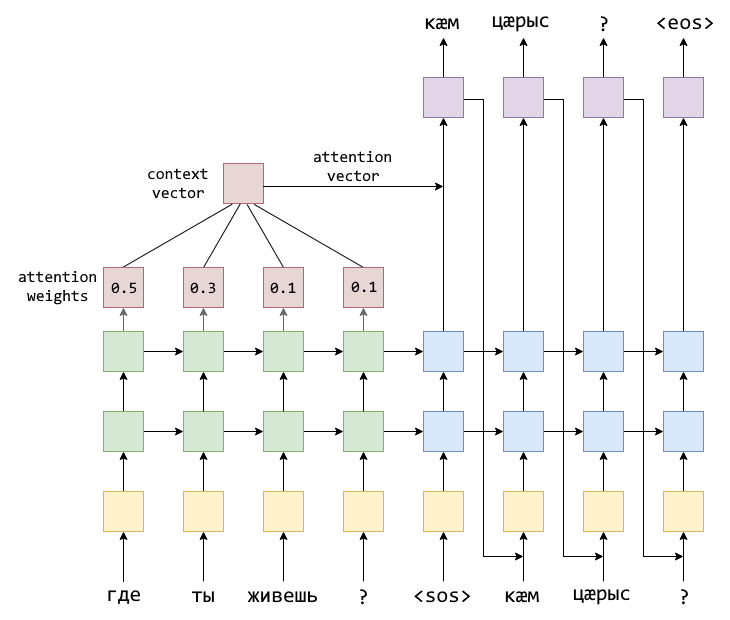
\includegraphics[width=0.75\textwidth]{img/Model.png}
		\caption{Encoder-Decoder Seq2Seq модель, с механизмом Attention}
	\end{figure}
	
	Последним этапом построение модели машинного перевода является определение механизма обучения. Нейронные модели Seq2Seq обучаются предсказывать распределения вероятностей следующего элемента последовательности с учетом предыдущего контекста. На каждом шаге нужно максимизировать вероятность, которую модель присваивает правильному элементу. 
	
	Формально, давайте представим, что у нас есть обучающий экземпляр с входом  $X = \{ x_0, ... , x_T \}$ и целевой выход $Y = \{ y_0, ... , y_T \}$. Затем на временном шаге $t$ модель предсказывает распределение вероятностей $P^{(t)} = P(*|y_0, ..., y_{t - 1}, x_0, ..., x_{T})$. Основная цель на этом этапе, чтобы модель присваивала вероятности 1 правильному элементу $y_t$ и 0 остальным.
	
	В таких случаях обычно использует максимальное логарифмическое правдоподобие (MLE) или категориальную кросс-энтропию (CCE) в качестве целевой функции обучения, которая является используемым методом оценки параметров распределения вероятностей. Формально, учитывая обучающий набор $ \mathcal{D} = \{\textlangle x(s), y(s) \textrangle\}_{s=1}^S $, целью обучения является поиск набора параметров модели $\theta$, которые максимизируют логарифмическую вероятность на обучающем наборе:
	
	$$
	    \hat{\theta}_{\text{loss}} = argmax(\mathscr{L}(\theta)),
	$$

    где логарифмическая вероятность определяется как:
    
    $$
      \mathscr{L(\theta)=\sum_{s=1}^S log(P(y^{(s)}|x^{(s)};\theta))}  
    $$
    
    Благодаря алгоритму обратного распространения ошибки можно эффективно вычислить градиент $\mathscr{L}$ относительно $\theta$ (параметров модели). При обучении моделей NMT обычно используется алгоритм стохастического градиентного спуска (SGD). Вместо вычисления градиентов на полном обучающем наборе SGD вычисляет функцию потерь и градиенты на маленькой части обучающего набора. Простой оптимизатор SGD обновляет параметры модели NMT с помощью следующего правила:
    
    $$
        \theta \leftarrow \theta - \alpha \nabla \mathscr{L}(\theta)
    $$
    
    где $\alpha$ - скорость обучения. При правильно выбранной скорости обучения параметры NMT гарантированно сходятся к локальному оптимуму. На практике оказывается, что адаптивные оптимизаторы скорости обучения, такие как Adam \cite{8}, значительно сокращают время обучения, а точность почти не снижается.
	
	\section*{Эксперимент}
	
	\subsection*{Датасет}
	
	Одним из главных аспектов для реализации хорошей модели перевода является качество и количество данных. Поэтому было принято решение проверять модели на двух датасетах. Больший датасет, содержащий пары русского и английского языка, даст возможность минимизировать ошибки в структуре построения. В свою очередь это увеличит шанс на удачную работу таких же моделей, но с другой парой языков. Второй датасет, содержащий пары русского и осетинского языка, гораздо меньше по размеру. Таким образом, можно сосредоточься только на параметрах моделей и этапах их обучения, при использовании такой связки пар языков.
    
    \begin{table}[h]
        \centering
        \begin{tabular}{|c|c|} 
        \hline
        \textbf{Тип языковой пары}                                       & \textbf{Количество}  \\ 
        \hline
        Русский язык $\shortrightarrow$ Английский язык & 100 000              \\ 
        \hline
        Русский язык $\shortrightarrow$ Осетинский язык & 1 878                \\
        \hline
        \end{tabular}
        \caption{Количество пар в датасетах}
    \end{table}
    
    
    Все материалы, который в последствие были использованы в качестве обучающих данных собраны на следующих ресурсах: 
	
	\begin{enumerate}
		\item Русский язык $\shortrightarrow$ Английский язык | \textit{RUS $\shortrightarrow$ ENG}:
		\begin{enumerate}
			\item ManyThings.org - Двуязычные Пары предложений, разделенные табуляцией. 
			Это выбранные пары предложений из проекта Tatoeba. \\ 
			\url{http://www.manythings.org/anki/}
		\end{enumerate}
		\item Русский язык $\shortrightarrow$ Осетинский язык | \textit{RUS $\shortrightarrow$ OSS} (Кусочно собран с разных ресурсов):
		\begin{enumerate}
			 \item Проект \textit{Tatoeba} - обширная база данных предложений и их переводов, постоянно пополняющаяся усилиями тясяч добровольных участников. \\ \url{https://tatoeba.org/ru/downloads}
			 \item Проект \textit{Биоингвӕтӕ} - Билингвы подготовлены для чтения с помощью электронных словарей программы Lingvo. \\ \url{https://ironau.ru/bilingva/index.htm}
			 \item Ф.М. Таказов - Краткий русско-осетинский разговорник. \\ \url{https://ironau.ru/takazov/phrasebook2.htm}
			 \item Ф.М. Таказов - Самоучитель осетинского языка. \\ \url{https://ironau.ru/takazov/index.htm}
 		\end{enumerate}
	\end{enumerate}
	
	\subsection*{Обработка данных}
	
    В процессе работы с данными были обнаружены некоторый перечень проблем. 
    
    Датасет \textit{RUS $\shortrightarrow$ ENG}, почти не имеет в себе проблем, кроме одной. В некоторых парах используется сокращения принятые в английском языке (Например: I am $\shortrightarrow$ I'm). Данная проблема не была решена. Поэтому в статье данная проблема игнорируется.
    
    Так же в датасете \textit{RUS $\shortrightarrow$ OSS} были обнаружены символы «æ» (Код: 1237) и «æ»(Код: 230). Данная буква несет в себе одинаковую смысловую нагрузку в языке, следовательно просто заменим все символы на «æ» с кодом 230 (т.к. аналогичный символ используется на Осетинской Википедии). 
    
    Еще есть проблема с символом «тире». Два вида символов «—» и «-», тоже несут в себе одинаковую ценность, связи с этим заменяем их на какое-то одно в данном случае на второй символ из представленных («-»).
    
    \subsection*{Обучение}
    
    Были созданы две модели. Первая модель перевода с русского языка на английский, вторая с русского на осетинский. Если более конкретно говорить о конфигурации моделей, то в качестве разновидности архитектуры RNN в блоках использована GRU \cite{4}. У моделей размер батча 64, размер Embedding слоя 256 токенов, количество эпох обучения является 15, функция потерь - Sparse Categorical Crossentropy. 
    
    \begin{table}[h]
    \centering
    \begin{tabular}{|l|l|c|} 
    \hline
    \multicolumn{1}{|c|}{\textbf{Параметр}} & \multicolumn{1}{c|}{\textbf{Переменная}}                 & \multicolumn{1}{c|}{\textbf{Значение}}  \\ 
    \hline
    \textit{Размер словаря} & \mintinline{python}{max_vocab_size} & 5000 \\ 
    \hline
    \textit{Размер Embedding слоя} & \mintinline{python}{embedding_dim} & 256 \\
    \hline
    \textit{Размерность выходного слоя} & \mintinline{python}{units} & 1024 \\
    \hline
    \textit{Количество эпох обучения выходного слоя} & \mintinline{python}{epochs} & 15 \\
    \hline
    \end{tabular}
    \caption{Используемые параметры моделей}
    \end{table}
    
    Непосредственно перейдем к рассмотрению модели и их результатов.
    
    Процедура обучения модели RUS-ENG заняла 1.5 часа на GPU NVidia RTX 2060 Super. На начальных этапах функция потерь имела значение около 7.462, но ошибка упала до значений ниже 2 после нескольких итераций. Последующие эпохи хоть и уменьшали значение, но не с такой скоростью, что была на начальном этапе. По окончанию обучения итоговая ошибка составляет 0.2056.
	
	\begin{figure}[h]
		\centering
		\captionsetup{justification=centering}
		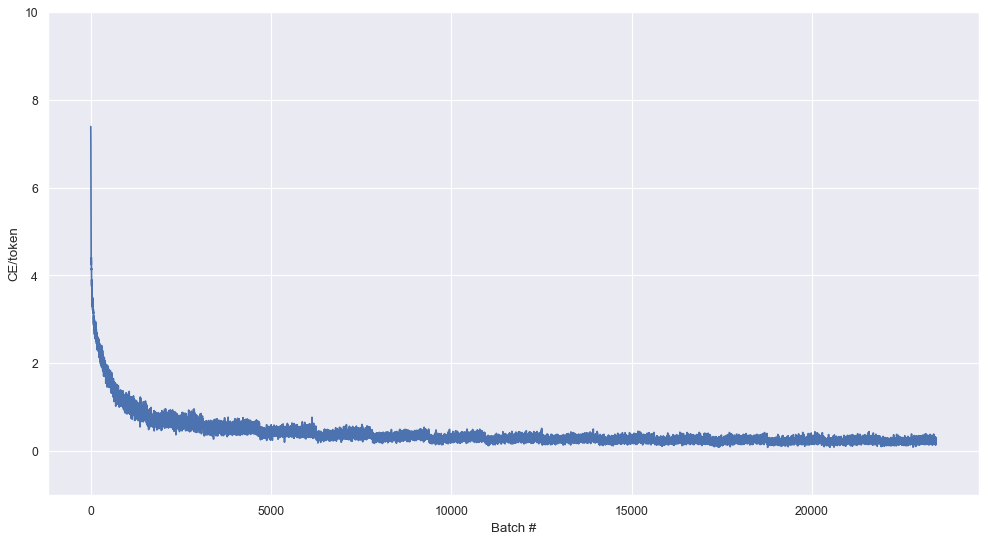
\includegraphics[width=0.9\textwidth]{img/RUS-ENG GRU-[1024]-Epochs[15]-EMD_DIM[256].png}
		\caption{ Падающий график функции потерь во время обучения [RUS-ENG]}
	\end{figure}
	
	В датасете основанном на паре русского и осетинского языков около 1800 пар предложений. Это означает, что время на обучение модели значительно уменьшится. Процедура обучения RUS-OSS с таким же GPU составила 0.5 часа.  Функция ошибка изначально находилась на отметке в 6.784 и после 15 эпох обучения упала до 0.217, что можно прекрасно увидеть на графике (Рис. 3).
	
	\begin{figure}[h]
		\centering
		\captionsetup{justification=centering}
		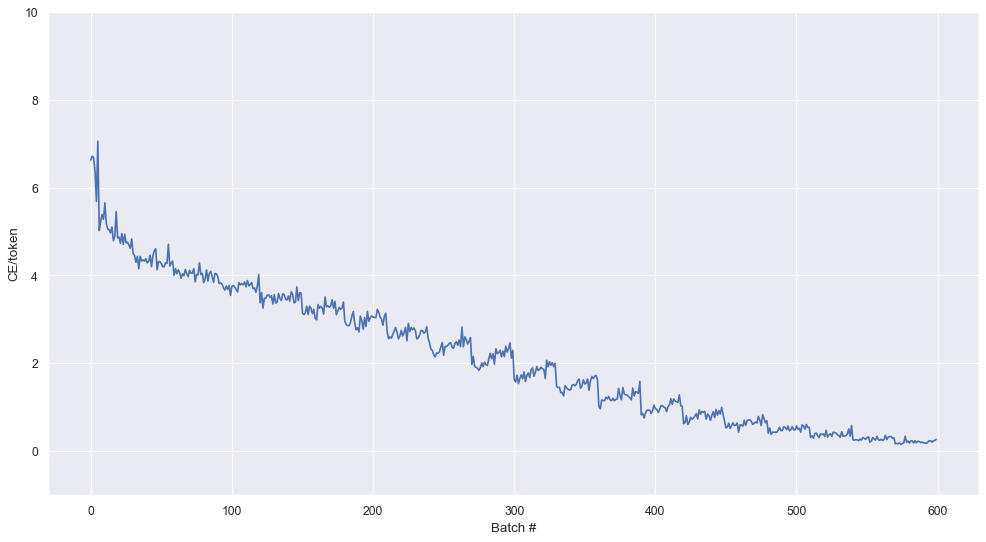
\includegraphics[width=0.9\textwidth]{img/RUS-OSS GRU-[1024]-Epochs[15]-EMD_DIM[256].png}
		\caption{ Падающий график функции потерь во время обучения [RUS-OSS] }
	\end{figure}
	
	\subsection*{Результат}
		
    Как оценить полученные модели? В качестве метрики качества перевода была выбрана BLEU \cite{9}. Выходные данные BLEU всегда представляют собой число от 0 до 1. Это значение указывает, насколько текст-кандидат похож на справочные тексты, при этом значения, близкие к 1, представляют более похожие тексты. BLEU будет считать на основе n-грамм размера 4.
	
	Посчитав средние значения BLEU-Score модели RUS-ENG, на текстовой выборки:
	
	\begin{table}[h]
        \centering
        \begin{tabular}{|c|c|} 
            \hline
            \textbf{Тип} & \textbf{Значение} \\ 
            \hline
            Среднее арифметическое & 0.50529 \\ 
            \hline
            Медиана & 0.45761 \\ 
            \hline
            Мода & 1 \\
            \hline
        \end{tabular}
        \caption{ [Model RUS-ENG] Средние значения BLEU-Score}
    \end{table}
    
    Полученные значение не особо дают ясности общей картине. Нельзя однозначно сказать, хорошая модель перевода у нас получилась или нет. 
    
    Тогда стоит рассмотреть сколько «хороших переводов» сгенерировала наша модель. Рассмотрим гистограмму по подсчету значений. В качестве абсциссы будет использоваться BLEU-Score одного предложения из тестовой выборки, ордината же в свою очередь представляет из себя количество. Высота полученных прямоугольников будет означать сколько всего было встречено предложений с одинаковым BLEU-Score.  Для большей наглядности округлим показатели BLEU-Score до одного знака после запятой.
	
	Смотря на полученный график (Рис. 4) видно, что довольно большая доля приходит на правильный перевод (BLUE-Score равный единице). В свою очередь весомая часть тестовой выборки дает, не однозначный показатель. По графику можно сказать, что почти больше половины предложений переведено «наполовину правильно».
    	
    \begin{figure}[h]
		\centering
		\captionsetup{justification=centering}
		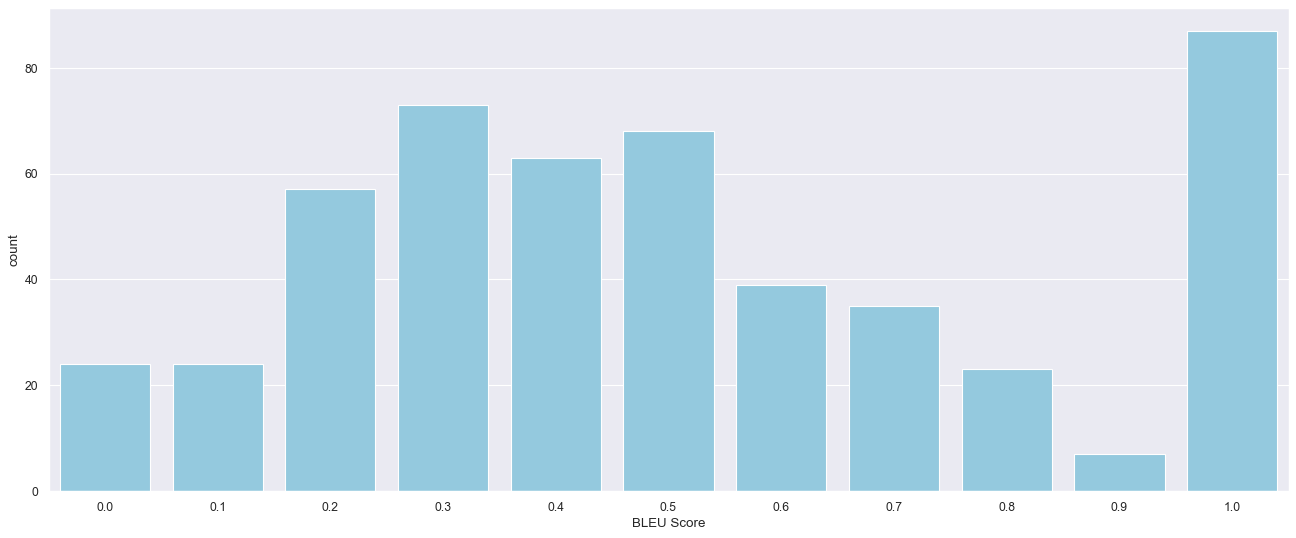
\includegraphics[width=0.8\textwidth]{img/RUS-ENG BLUE Score RUS-ENG Epochs-15.png}
		\caption{ [Model RUS-ENG] Гистограмма BLUE-Score для тестовой выборки}
	\end{figure}
	
	Само собой BLUE-Score довольно хорош в измерение качества перевода, однако стоит и рассмотреть конкретные примеры перевода.
	
	Входное предложение «\textit{Открывай панель.}». Модель выдает такой результат:
	\begin{table}[h]
	\footnotesize {
        {Orginal}: Открывай панель. \\
        {Human Translation}: open the panel . \\
        {Machine Translation}: open the cage . \\
        {BLEU 4-gram}: 0.5791460926441345
    }
	\end{table}
	
	На месте, где должно быть слово «\textit{panel}» находится «\textit{cage}». Связано это с тем, что в словаре модели просто нет слова «\textit{панель}» и соответственно его перевода тоже. В таких случаях модель может выдавать абсолютно случайны перевод. 
	
	\begin{figure*}[ht!]
        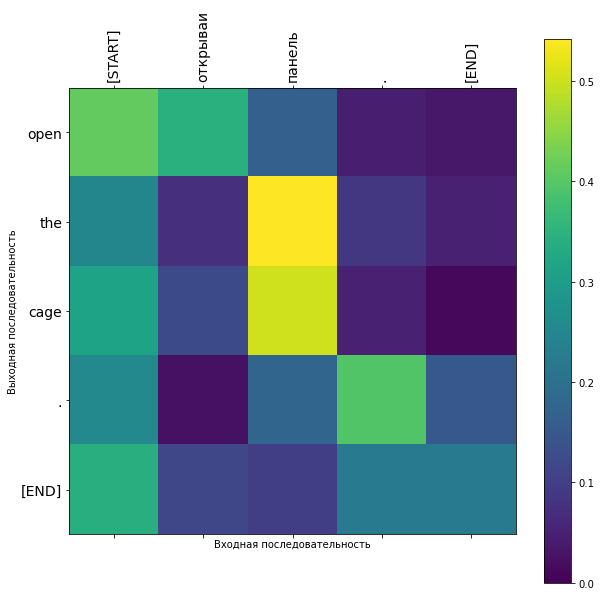
\includegraphics[width=.5\textwidth]{img/RUS-ENG-1.png}\hfill
        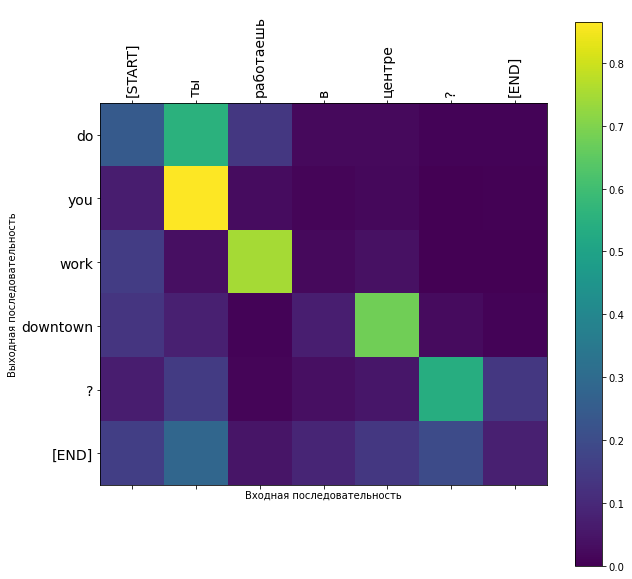
\includegraphics[width=.5\textwidth]{img/RUS-ENG-2.png}\hfill
        \caption{(Левый) «Открывай панель.» (Правый) «Ты работаешь в центре?»}
    \end{figure*}
	
	Исходя из этого можно сделать вывод, что структуру предложений, при наличие необходимого количества данных модель, распознает и генерирует сама. Однако если в словаре не оказалось, слов, которые требуют перевода, модель ведет себя непредсказуемо. 
	
	Давайте рассмотрим более удачный перевод. Предложение «Ты работаешь в центре?». 
	
	\begin{table}[h]
	\footnotesize {
    	{Orginal}: Ты работаешь в центре? \\
        {Human Translation}: do you work downtown ? \\
        {Machine Translation}: do you work downtown ? \\
        {BLEU 4-gram}: 1.0
    }
    \end{table}

    Модель довольно хорошо справилась с правилами построения вопроса на английском языке. Отсюда можно утверждать, что подбор «правильных» данных при обучении, сильно способствует улучшению качества модели.
    
    На правой диаграмме (Рис.5), довольно хорошо видно, что хоть первое слово на вход это местоимение «\textit{ты}», модель выдает большую вероятность на конструкции «\textit{do you}», за счет обработки механизма Attetion. Так же игнорирует предлог «\textit{в}», и вовсе его не переводит. 
    
    Напрашивается вывод, что качество модели напрямую зависит от датасета, на котором она обучается. Сама модель довольно хорошо справляется с моделированием нюансов языка, на котором обучалась.
	
	Давайте так же рассмотрим модель с парами русского и осетинского языков (\textit{RUS $\shortrightarrow$ OSS}). Взглянув на гистограмму по подсчету значений BLUE-Score можно сразу заметить, что количество абсолютно неправильных переводов больше в разы по соотношению с неправильными, в отличии от предыдущей модели. Промежуточные показатели выглядят абсолютно не существенно по отношению к значениям BLUE равных нулю и единице.
	
	\begin{figure}[h]
		\centering
		\captionsetup{justification=centering}
		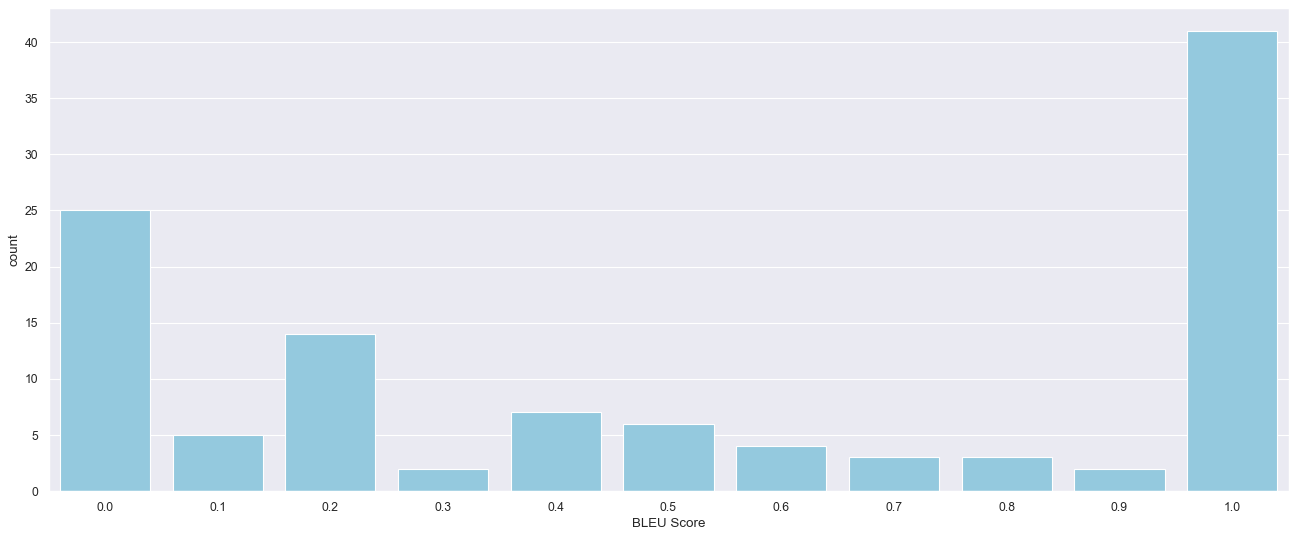
\includegraphics[width=0.8\textwidth]{img/RUS-OSS BLUE Score RUS-ENG Epochs-15.png}
		\caption{ [Model RUS-OSS] Гистограмма BLUE-Score для тестовой выборки}
	\end{figure}
    
    Посчитаем такие же средние значения для текущей модели:
    
	\begin{table}[h]
        \centering
        \begin{tabular}{|c|c|} 
            \hline
            \textbf{Тип} & \textbf{Значение} \\ 
            \hline
            Среднее арифметическое & 0.5555 \\ 
            \hline
            Медиана & 0.6019 \\ 
            \hline
            Мода & 1 \\
            \hline
        \end{tabular}
        \caption{ [Model RUS-OSS] Средние значения BLEU-Score}
    \end{table}
    
    Сразу видно, что средние показатели выше, по сравнению с моделью RUS-ENG, но качество перевода все равно ниже. Хоть и значения модели выглядят лучше, но по оценке BLEU перевод все равно хуже. Как же так получается? На самом деле такое сравнение не совсем корректно, потому что количество пар предложений на которых модели обучались довольно сильно отличаются. Средние значения почти никакой конкретной информации нам не дают.
    
    Поэтому всегда после общих оценок стоит рассмотреть конкретные переводы и сравнить их качество и постараться выделить некоторые особенности. 
	
	\begin{figure*}[ht!]
        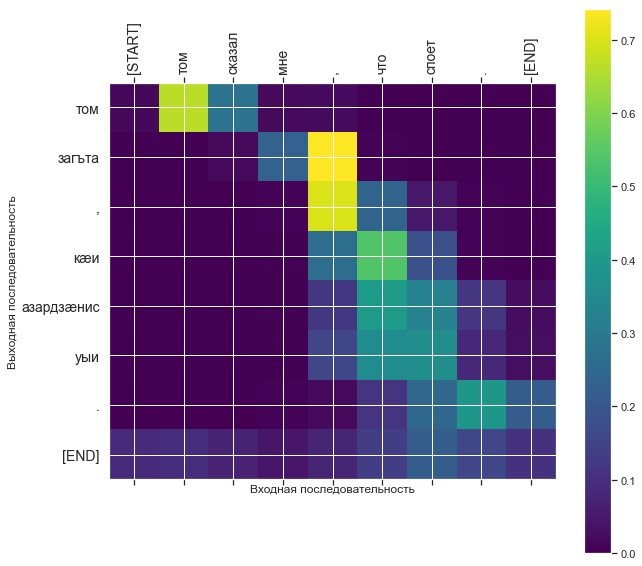
\includegraphics[width=.5\textwidth]{img/RUS-OSS-5.png}\hfill
        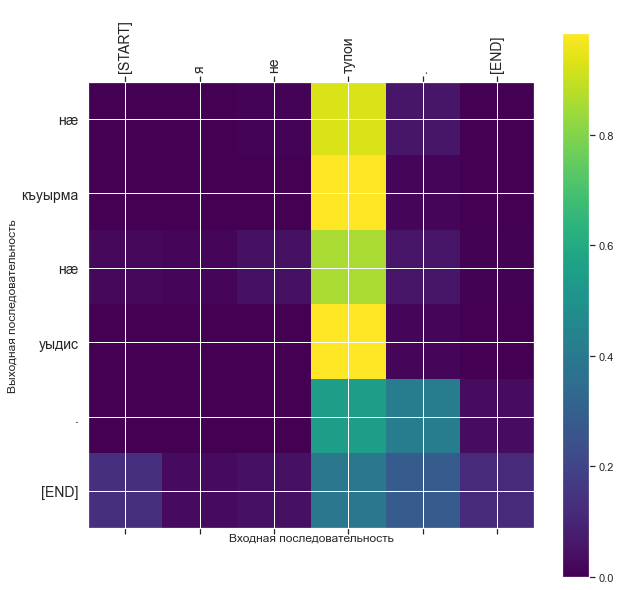
\includegraphics[width=.5\textwidth]{img/RUS-OSS-3.png}\hfill
        \caption{Attention. (Левый) «Том сказал мне, что споёт.» (Правый) «Я не тупой.»}
    \end{figure*}
    
	\begin{table}[h]
	\footnotesize {
    	{Orginal}:  Том сказал мне, что споёт. \\
        {Human Translation}: том мын загъта , кæи азардзæнис уыи . \\
        {Machine Translation}: том загъта , кæи азардзæнис уыи . \\
        {BLEU 4-gram}: 0.8649141545451661
    }
    \end{table}
    
    На левом Рис. 7 видно, что модель не особо придала значение местоимению «\textit{мне}» и не перевело его. Оценка BLEU, хоть и не является идеальной, но смысл переводимого предложения остается верным. Так же видно, что структура построения осетинского предложения и русского гораздо ближе, чем между русским и английским, поэтому на графике можно заметить, что большие вероятности расположены на диагонали. Это говорит о том, что перевод происходит почти дословно. 
    
    Второй же случаи показывает, что модель не справляется с предложениями как хотелось бы.
    
    \begin{table}[h]
	\footnotesize {
    	{Orginal}:  Я не тупой. \\
        {Human Translation}: æз къуырма нæ дæн . \\
        {Machine Translation}: нæ къуырма нæ уыдис . \\
        {BLEU 4-gram}: 0.5999350121649039
    }
    \end{table}
    
    Хоть предложение и переведено по оценки BLEU почти на 50\% верно, но смысл фразы потерялся полностью. На диаграмме (Правый Рис. 7), мы видим не диагональную подсветку вероятностей, а почти вертикальную прямую. Это говорит о том, что модель посчитала только одно слово «тупой» как особо важное и почти все предложение переводило учитывая контекст только этого слова.
    
    Основываясь на построенных моделях, можно сказать, что качество модели не только зависит от параметров самой модели, но и от данных на которых она обучалась. Модель обученная на данных RUS-ENG получилась гораздо лучше, чем модель на данных RUS-OSS.
    
    
    \section*{Вывод}
    
    Нейронный машинный перевод стал доминирующим подходом к машинному переводу как в исследованиях, так и на практике. В этой статье были рассмотрены широко используемые методы в NMT, включая моделирование, декодирование, интерпретацию, а также оценку данных. 
    
    Несмотря на большой успех, достигнутый NMT, все еще остается много проблем, которые необходимо изучить. Одна из таких это попытки интерпретировать NMT, такая проблема все еще актуальна. Понимание того, как и почему нейронный машинный перевод выдает такой результат, важно для определения недостатков и неточностей NMT.
    
    Исходя из проведенных экспериментов с разными моделями машинного перевода, можно сделать вывод концепция Seq2Seq нейронного перевода, довольно хорошо справляется с построением правильного с точки зрения смысла и грамматики перевода, однако на прямую зависит от качество обучаемых данных.
    
	\clearpage
	
	\addcontentsline{toc}{section}{Список используемой литературы}
	
	\begin{thebibliography}{}
	    \footnotesize {
		\bibitem{1}  S. Hochreiter, J. Schmidhuber	-	Long Short-Term Memory; 1997.
		
		\url{https://www.researchgate.net/publication/13853244_Long_Short-term_Memory}
		
		\bibitem{2}  Junyoung Chung, Caglar Gulcehre, KyungHyun Cho, Yoshua Bengio	-	Empirical Evaluation of Gated Recurrent Neural Networks on Sequence Modeling; 2014.
		
		\url{https://www.researchgate.net/publication/269416998_Empirical_Evaluation_of_Gated_Recurrent_Neural_Networks_on_Sequence_Modeling}
		
		\bibitem{3} Ilya Sutskever	-	Training recurrent neural networks; 2013.
		
		\url{https://www.cs.utoronto.ca/~ilya/pubs/ilya_sutskever_phd_thesis.pdf}
		
		\bibitem{4} Ri Wang, Maysum Panju, Mahmood Reza Gohari -   Classification-based RNN machine translation using GRUs; 2017
		
		\url{https://www.researchgate.net/publication/315570520_Classification-based_RNN_machine_translation_using_GRUs}
		
		\bibitem{5} Tomohiro Fujita, Zhiwei Luo, Changqin Quan, Kohei Mori - Simplification of RNN and Its Performance Evaluation in Machine Translation; 2020
		
		\url{https://www.jstage.jst.go.jp/article/iscie/33/10/33_267/_pdf/-char/en}
		
		\bibitem{6} Sainik Kumar Mahata, Dipankar Das and Sivaji Bandyopadhyay -  MTIL2017: Machine Translation Using Recurrent Neural Network on Statistical Machine Translation; 2018
		
		\url{https://www.researchgate.net/publication/325456613_MTIL2017_Machine_Translation_Using_Recurrent_Neural_Network_on_Statistical_Machine_Translation}
		
		\bibitem{7} Zhixing Tan, Shuo Wang, Yang Zonghan, Gang Chen - Neural Machine Translation: A Review of Methods, Resources, and Tools; 2020
		
		\url{https://www.researchgate.net/publication/348079690_Neural_Machine_Translation_A_Review_of_Methods_Resources_and_Tools}
		
		\bibitem{8} Timothy Mayer, Ate Poortinga, Biplov Bhandari, Andrea P. Nicolau, Kel Markert, Nyein Soe Thwal, Amanda Markert, Arjen Haag, John Kilbrideh, Farrukh Chishtie, Amit Wadhwai, Nicholas Clintonj, David Saah - Deep Learning approach for Sentinel-1 Surface Water Mapping leveraging Google Earth Engine; 2021
		
		\url{https://www.researchgate.net/publication/355005296_Deep_Learning_approach_for_Sentinel-1_Surface_Water_Mapping_leveraging_Google_Earth_Engine}
		
		\bibitem{9} Kishore Papineni, Salim Roukos, Todd Ward, Wei-Jing Zhu - BLEU: a Method for Automatic Evaluation of Machine Translation; 2002
		
		\url{https://www.researchgate.net/publication/2588204_BLEU_a_Method_for_Automatic_Evaluation_of_Machine_Translation}
		
		\bibitem{10} Ashish Vaswani, Noam Shazeer, Niki Parmar, Jakob Uszkoreit, Llion Jones, Aidan N. Gomez, Lukasz Kaiser, Illia Polosukhin - Attention Is All You Need
		
		\url{https://arxiv.org/abs/1706.03762}
		
		\bibitem{11} Mani Wadhwa - seq2seq model in Machine Learning, 2021
		
		\url{https://www.geeksforgeeks.org/seq2seq-model-in-machine-learning/}
		}
	\end{thebibliography}
\end{document}


% \begin{lstlisting}[language=iPython]

% \end{lstlisting}